% Style for a MSc paper at Warsaw School of Economics
% Michał Ramsza
% Friday, December 14, 2012

% --- document class and other global stuff ---------------------------
\documentclass[polish, twoside, 12pt, a4paper]{article}

%% --- packages --------------------------------------------------------
\usepackage{textcomp}
\usepackage{times}
\usepackage{amsmath}
\usepackage{amsfonts}
\usepackage{amssymb}
\usepackage{amsthm}
\usepackage[T1]{fontenc}
\usepackage[utf8]{inputenc}
\usepackage{graphicx}
\usepackage{xcolor}
\usepackage{enumitem}
\usepackage[polish]{babel}
\usepackage[centering, left=3.5cm, right=2.5cm, textheight=24cm]{geometry}
\usepackage{csvsimple}
\usepackage[T1]{fontenc}
% --- packages for citations ------------------------------------------
\usepackage[square,numbers]{natbib}
\AtBeginDocument{\renewcommand{\harvardand}{i}}

% --- package for automatic insertion of R code -----------------------
\usepackage{listings}
\lstset{language=R,%
   numbers=left,%
   tabsize=3,%
   numberstyle=\footnotesize,%
   basicstyle=\ttfamily \footnotesize \color{black},%
   escapeinside={(*@}{@*)}}

\begin{filecontents*}{grade.csv}
name,givenname,matriculation,gender,grade
Maier,Hans,12345,m,1.0
Huber,Anna,23456,f,2.3
Weisbaeck,Werner,34567,m,5.0
\end{filecontents*}


% --- support for links -----------------------------------------------
\usepackage{url}
\usepackage{hyperref}
\hypersetup{colorlinks=true,
            linkcolor=black,
            citecolor=darkgray,
            urlcolor=darkgray,
            pagecolor=darkgray}

% --- support for large tables and other stuff ------------------------
\usepackage{longtable}
% \usepackage{subfigure} % this package will not work with subcaption package
\usepackage{float}
\usepackage{caption}
\usepackage{subcaption}
\usepackage{wrapfig}
\usepackage{pdflscape} % relevant for wide tables (rotating pages)

% --- packages for game theory -----------------------------------------
\usepackage{sgame}

% --- support for no widows --------------------------------------------
\usepackage[defaultlines=4,all]{nowidow}

% --- quotation for polish language \enquote{}
\usepackage[autostyle]{csquotes}
\DeclareQuoteAlias{dutch}{polish}

% --- definitions for environments -------------------------------------
\theoremstyle{definition}
    \newtheorem{condition}{Założenie}
    \newtheorem{example}{Przykład}

\theoremstyle{plain}
    \newtheorem{definition}{Definicja}
    \newtheorem{proposition}{Stwierdzenie}
    \newtheorem{theorem}{Twierdzenie}
    \newtheorem{cor}{Wniosek}

\theoremstyle{remark}
    \newtheorem{remark}{Uwaga}

% --- other settings --------------------------------------------------
\linespread{1.5}
\frenchspacing
\sloppy
\allowdisplaybreaks[4]
\raggedbottom
\clubpenalty=10000
\widowpenalty=10000

% --- only if required ------------------------------------------------
\AtBeginDocument{\renewcommand*{\figurename}{Wykres}}
\AtBeginDocument{\renewcommand*{\tablename}{Tabela}}

% --- changing definition of footnote ---------------------------------
\makeatletter
\renewcommand\footnotesize{%
   \@setfontsize\footnotesize\@ixpt{10}%
   \abovedisplayskip 8\p@ \@plus2\p@ \@minus4\p@
   \abovedisplayshortskip \z@ \@plus\p@
   \belowdisplayshortskip 4\p@ \@plus2\p@ \@minus2\p@
   \def\@listi{\leftmargin\leftmargini
               \topsep 4\p@ \@plus2\p@ \@minus2\p@
               \parsep 2\p@ \@plus\p@ \@minus\p@
               \itemsep \parsep}%
   \belowdisplayskip \abovedisplayskip
}
\makeatother


% ---------------------------------------------------------------------
\begin{document}

% --- strona tytulowa -------------------------------------------------
\begin{titlepage}
\centering


\includegraphics[width=0.66\textwidth]{logo.JPG}

\vspace*{0.5cm}
Studium magisterskie\\
\begin{flushleft}
Kierunek: Metody Ilościowe w Ekonomii i Systemy Informacyjne\\
%Specjalność: <specjalność>
% Forma studiów: <forma studiów (stacjonarne, itd.)>
\end{flushleft}

\vspace*{.5cm}
\rule{0cm}{1cm}\hfill
\begin{minipage}{9cm}
Imie i nazwisko autora: Oskar Furmańczuk\\
Nr albumu: 81794
\end{minipage}

\vspace*{1cm}
\begin{minipage}{12cm}
\centering
\Large
\textbf{Determinanty przebiegu choroby COVID-19.}
\end{minipage}

\vspace*{2cm}
\rule{0cm}{1cm}\hfill
\begin{minipage}{9cm}
Praca magisterska napisana\\
w Katedrze Matematyki i Ekonomii Matematycznej\\
pod kierunkiem naukowym\\
dr hab. Michała Ramszy
\end{minipage}

\vfill
Warszawa 2021
\end{titlepage}

\rule{1ex}{0ex}\clearpage

\graphicspath{ {./images/} }
% --- table of contents -----------------------------------------------
\cleardoublepage
\tableofcontents

% --- chapter ---------------------------------------------------------
\cleardoublepage
\section{Wprowdzenie}

%- przegląd litertury dotyczącej koronawirusa - artykuły poświęcone badaniom wpływu czynników biologicznych na przebieg choroby \\
%- związek pracy z ekonomią \\

\subsection{Tło oraz problem badawczy}

Rok 2020 z pewnością zostanie zapisany na kartach historii jako rok rozpoczęcia jednej z największych pandemii jaka dotknęła naszą cywilizację. Wirus SARS-CoV-2, wywołujący chorobę COVID-19, pozbawił życia milionów ludzi w każdym zakątku naszej planety. Oprócz strat w postaci ofiar śmiertelnych pandemia COVID-19 spowodowała istotne zmiany we wszystkich gałęziach światowej gospodarki. Globalna pandemia zachwiała parkietami giełdowymi, nasiliła fluktuacje na rynku pracy oraz wpłynęła na sytuację finansową wielu przedsiębiorstw i gospodarstw domowych. Niestety, większość z tych następstw miała negatywny, a czasem destruktywny w skutkach finał. Z powodu surowych obostrzeń, ustalanych w celu walki z epidemią, wiele osób straciło zatrudnienie oraz liczne przedsiębiorstwa ogłosiły upadłość. Z kolei te następstwa spowodowały częste problemy ze spłatami zaciągniętych zobowiązań kredytowych. Władzę dotkniętych kryzysem krajów zostały również zmuszone do modyfikacji polityki budżetowej i monetarnej.  

W celu ograniczenia tych wyniszczających procesów niezbędne jest opracowanie efektywnej strategii walki z epidemią. Jedną ze składowych takiej strategii mogłoby stać się wyselekcjonowanie osób najbardziej narażonych na ciężki przebieg tej choroby. Grupa tych osób mogłaby zostać objęta wzmożoną obserwacją w celu zapewnienia im intensywnej opieki medycznej w przypadku wykrycia wirusa SARS-CoV-2 w ich organizmie. Przez zmniejszenie ryzyka prawdopodobieństwa poniesienia wysokich strat w ofiarach śmiertelnych możliwy byłby powrót do sposobu funkcjonowania gospodarki sprzed pandemii. 

Do przeprowadzenia opisanej selekcji niezbędne byłoby wyodrębnienie zestawu cech umożliwiających właściwe rozpoznanie osób z grupy podwyższonego ryzyka. W czasie sporządzania tej pracy nie istniał tak ustandaryzowany zbiór zmiennych.

\subsection{Cel i hipoteza badawcza}

Głównym celem pracy jest przedstawienie argumentów na rzecz hipotezy, że możliwe jest określenie zbioru zmiennych, które w istotny sposób determinują przebieg choroby COVID-19. Istotność definiowana jest przez zestawienie otrzymanych miar stopnia determinacji przebiegu choroby przez wybrane zmienne z wynikami uzyskanymi przez losowy wybór. Przebieg zachorowania zostanie ograniczony do dwóch stanów: \emph{Ozdrowienie} - w przypadkach powrotu do zdrowia oraz \emph{Zgon} - w przypadkach gdy choroba zakończyła się zgonem.

Kolejnym celem badania jest określenie poziomu oraz kierunku wpływu wybranych cech na przebieg choroby. Zarówno ten jak i poprzedni punkt zostanie opracowany za pośrednictwem, skonstruowanego na tą potrzebę, modelu uczenia maszynowego. Ostatnim celem pracy będzie przedstawienie literatury z zakresu badań nad COVID-19 oraz opisanie wybranych metod i miar wykorzystywanych w uczynieniu maszynowym. 

\subsection{Organizacja pracy}

Praca dyplomowa pod tytułem \emph{Determinanty przebiegu choroby COVID-19} złożona jest z 6 rozdziałów. Struktura została opracowana w klasycznym akademickim podejściu, a charakter pracy można sklasyfikować jako empiryczny.

Rozdział \emph{Przegląd literatury} przybliża opracowane do tej pory badania zajmujące się opisem przebiegu choroby COVID-19. Przytoczone w nim badania poruszają tematykę wpływu cech biologicznych i zmiennych środowiskowych na proces rekonwalescencji pacjentów z wykrytym COVID-19.

W rozdziale \emph{Opis zbioru danych} zostały zdefiniowane użyte w pracy zbiory danych. Przedstawiono ich pochodzenie, wykonane na nich operacje oraz potencjalne trudności mogące wyniknąć z ich użycia. W tym rozdziale opisano także charakter i własności użytych zmiennych.

Rozdział \emph{Metody} zawiera opis wszystkich technik jakie zostały użyte na etapach przygotowania danych, tworzenia modelu oraz jego interpretacji. Opisano wybrane metody z zakresu uczenia maszynowego oraz uargumentowano istotę ich użycia w tej pracy.

W rozdziale \emph{Wyniki i dyskusja} zostały zebrane wartości wszystkich istotnych miar jakie uzyskano przy budowie, walidacji i interpretacji modelu. Opracowano także wnioski płynące z tych miar. Następnie porównano otrzymane wyniki z wnioskami badań przywołanych w rozdziale \emph{Przegląd literatury}.

Ostatni rozdział, czyli \emph{Zakończenie} zwiera podsumowanie pracy. Opracowane w nim zostały wnioski płynące z pracy oraz możliwe ich wykorzystanie w innych badaniach.


% --- chapter ---------------------------------------------------------
\cleardoublepage
\section{Przegląd literatury}
\label{chapter:przeglad-literatury}
\subsection{Rasa jako determinanta przebiegu choroby COVID-19 u pacjentów z chorobą współistniejącą}

Jednym z projektów prowadzonych na rzecz opisu przebiegu COVID-19 u pacjentów pochodzących z różnych grup rasowych jest „Racial disparities in patients with coronavirus disease 2019 infection and gynecologic malignancy”. Badanie to zostało przeprowadzone w Stanach Zjednoczonych na podstawie danych zebranych przez osiem systemów nowojorskich szpitali w okresie od 1 marca 2020 do 20 maja 202. Celem tego badania było sprawdzenie, czy istnieją rozbieżności na tle rasowym wśród pacjentek z rakiem ginekologicznym, u których stwierdzono obecność COVID-19.Wszystkie pacjentki biorące udział w badaniu miały ukończone 18 lat. Porównano charakterystykę wyjściową i kliniczną, zbadano różnice we wskaźnikach hospitalizacji i śmiertelności oraz wpływ rasy i innych czynników socjoekonomicznych i zdrowotnych na wyniki związane z COVID-19. 

Charakterystyka pacjentów obejmowała wiek, podawaną przez siebie rasę i pochodzenie etniczne, hrabstwo zamieszkania, status zatrudnienia, status pracownika zasadniczego, status ubezpieczenia, status mieszkaniowy, medyczne choroby współistniejące, ciężkość zakażenia COVID-19, typ raka, stadium rozpoznania, aktualny stan choroby nowotworowej i ostatnie leczenie przeciwnowotworowe.  Charakterystyka kliniczna COVID-19 obejmowała objawy COVID-19, parametry życiowe przy początkowym stadium choroby, powikłania szpitalne z powodu COVID-19 i konieczność stosowania dodatkowego tlenu, w tym inwazyjnej wentylacji mechanicznej. 

Rasę sklasyfikowano jako 2 grupy: czarnoskórzy versus nie-czarnoskórzy (biali plus pozostali). Zgrupowano pacjentów, którzy identyfikowali się jako Azjaci, Amerykańscy Indianie lub Rdzenni mieszkańcy Alaski, a także rdzenni Hawajczycy lub mieszkańcy Wysp Pacyfiku do innej grupy ze względu na niską liczbę w każdej kategorii. Biorąc pod uwagę wysoki odsetek białych w grupie innej niż czarna, rasy następnie podzielono na trzy grupy - czarnoskórzy, biali oraz pozostali. Łącznie 193 pacjentów - 67 czarnoskórych oraz 126 pozostałych.

Statystyki opisowe zostały obliczone dla cech demograficznych, socjoekonomicznych, zdrowotnych, związanych z nowotworem oraz związanych z COVID-19 u pacjentów rasy czarnej i innej niż czarna. Zmienne ciągłe zostały opisane jako mediany i przedziały międzykwartylowe (IQR) i zostały porównane między grupami za pomocą testu sumy rang Wilcoxona. Zmienne kategoryczne przedstawiono jako częstości i proporcje, a następnie zostały porównane między grupami za pomocą testu chi kwadrat. Wskaźniki hospitalizacji i śmiertelności obliczono wśród pacjentów rasy czarnej i innej niż czarna w populacji ogólnej lub w subpopulacji stratyfikowanej przez inne zmienne kategoryczne, a następnie porównano je za pomocą testu chi kwadrat.
	
Analiza wyników wykazała, iż nad 70\% pacjentów rasy czarnej w tym badaniu wymagało hospitalizacji z powodu zakażenia COVID-19, w porównaniu z zaledwie 46\% pacjentów rasy innej niż czarna. Oprócz rasy i wieku, zły stan sprawności i większa liczba chorób współistniejących wiązały się ze zwiększonym prawdopodobieństwem przyjęcia do szpitala. W szczególności, pacjenci rasy czarnej w wieku poniżej 65 lat prawie 5 razy częściej wymagali hospitalizacji z powodu COVID-19 w porównaniu z pacjentami rasy czarnej w tym samym wieku. Rasa czarna nie była związana ze zwiększoną śmiertelnością z powodu COVID-19 przed lub po skorygowaniu o cechy kliniczne i socjoekonomiczne. Badanie wykazało, że pacjenci rasy czarnej są od 2 do 3 razy bardziej narażeni na konieczność hospitalizacji niż pacjenci rasy białej po skorygowaniu czynników zakłócających, w tym wieku, płci, chorób współistniejących i dochodów, a prawdopodobieństwo ich śmierci z powodu zakażenia COVID-19 jest ponad 5 razy większe.

%---obrazek---------
\begin{figure}[h]
\centering
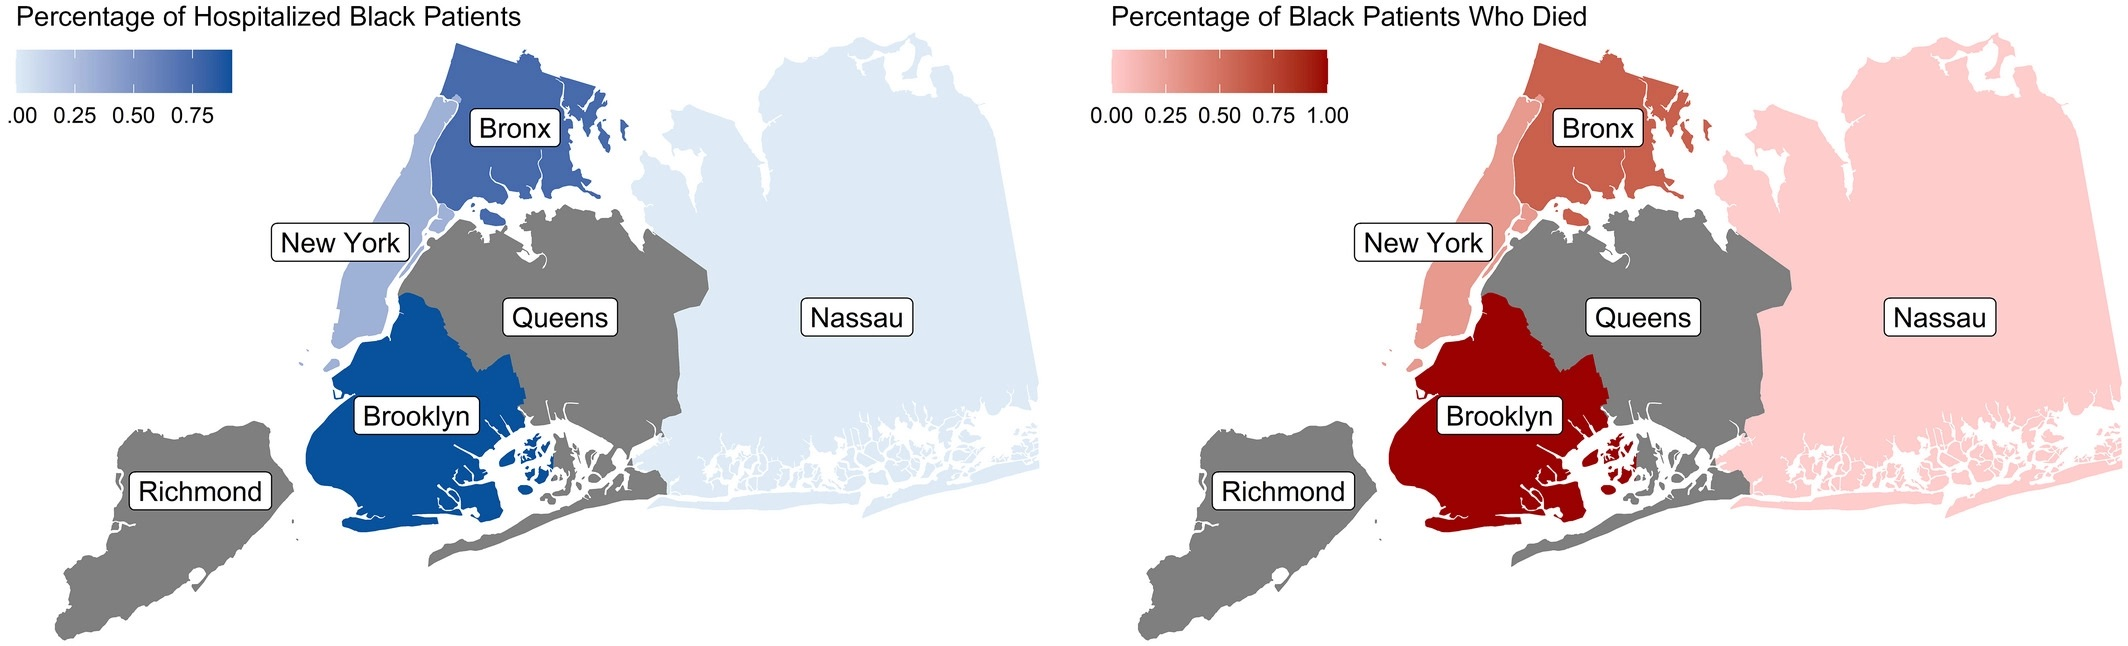
\includegraphics[width=15cm]{NY-racial-disparities.jpg}
\caption{Odsetki hospitalizacji (po lewej) i dane dotyczące śmiertelności (po prawej) zilustrowane dla pacjentów rasy czarnej w badanych dzielnicach Nowego Yorku (USA)}
\end{figure}

Autorzy badania wskazują za przyczynę gorszych rokowań czarnoskórych czynniki takie jak ograniczony dostęp do świadczeń opieki zdrowotnej, strukturalne i społeczne uwarunkowania opieki medycznej, rasizm i dyskryminację. Ponadto, Afroamerykanie są bardziej narażeni na współistniejące choroby medyczne, o których wiadomo, że są czynnikami ryzyka ciężkiego zakażenia COVID-19, w tym nadciśnienie tętnicze, cukrzycę, choroby nerek i układu oddechowego. W tej grupie badawczej większy odsetek czarnych pacjentów w wieku poniżej 65 lat miał więcej niż 3 współistniejące choroby i charakteryzował się większą częstością występowania nadciśnienia tętniczego, otyłości i cukrzycy w porównaniu z pacjentami rasy innej niż czarna w tej grupie wiekowej. Czarnoskórzy pacjenci mieli również częściej zamieszkiwali obszary poniżej granicy ubóstwa. \cite{borghesi2020}

\subsection{Wpływ wieku oraz płci na przebieg COVID-19}

Jednym z badań które zgłębia przebieg infekcji COVID-19 u pacjentów różnej płci z podziałem na grupy wiekowe jest \emph{Radiographic severity index in COVID-19 pneumonia: relationship to age and sex in 783 Italian patients}. Badnie zostało przeprowadzone na grupie 783 (532 mężczyzn i 251 kobiet) włoskich pacjentów z laboratoryjnie stwierdzonym COVID-19. Osoby poniżej 20 roku życia zostali wykluczeni z badania. Pozostali pacjenci zostali podzieleni na 7 grup wiekowych: 20-29 lat (grupa A), 30-39 lat (grupa B), 40-49 lat (grupa C), 50-59 lat (grupa D), 60-69 lat (grupa E), 70-79 lat (grupa F) oraz powyżej 80 lat (grupa G). Do interpretacji stanu pacjenta posłużono się osiemnasto-poziomowym wskaźnikiem oceny sprawności płuc uzyskiwanym przez analizę prześwietleń klatki piersiowej (dalej: CXR).

Mediana wieku wynosiła 65 lat (zakres międzykwartylowy, 55-74 lata). Spośród włączonych pacjentów, 10 (1,3\%) było z grupy A, 29 (3,7\%) z grupy B, 80 (10,2\%) z grupy C, 168 (21,5\%) z grupy D, 196 (25\%) z grupy E, 210 (26,8\%) z grupy F i 90 (11,5\%) z grupy G. Dla każdej grupy, test Manna-Whitneya U został użyty do porównania wyników CXR mężczyzn i kobiet. Korelacja rang Spearmana została zastosowana do oceny zależności pomiędzy wynikiem CXR a wiekiem. Test Kruskala-Wallisa zastosowano również w celu określenia, czy istnieją istotne różnice w punktacji CXR pomiędzy grupami wiekowymi. Wartości p $\leq$ 0,05 uznano za istotne statystycznie.

Wynik CXR był istotnie wyższy u mężczyzn niż u kobiet tylko w grupach D, E i F (p < 0,020). Stwierdzono istotną korelację między wynikiem CXR a wiekiem zarówno u mężczyzn, jak i u kobiet (rho = 0,205, p < 0,0001 dla mężczyzn; rho = 0,310, p < 0,0001). U mężczyzn wynik CXR w grupach D, E, F i G był znamiennie wyższy niż w grupach A, B i C (ryc. 3). U kobiet wynik CXR w grupach E, F i G był znamiennie wyższy niż w grupach A i B (ryc. 3). Wynik CXR w grupie G był również znamiennie wyższy niż w grupach C, D i E. Wynik CXR w grupie F był znamiennie wyższy niż w grupie C.

\begin{figure}[h]
\centering
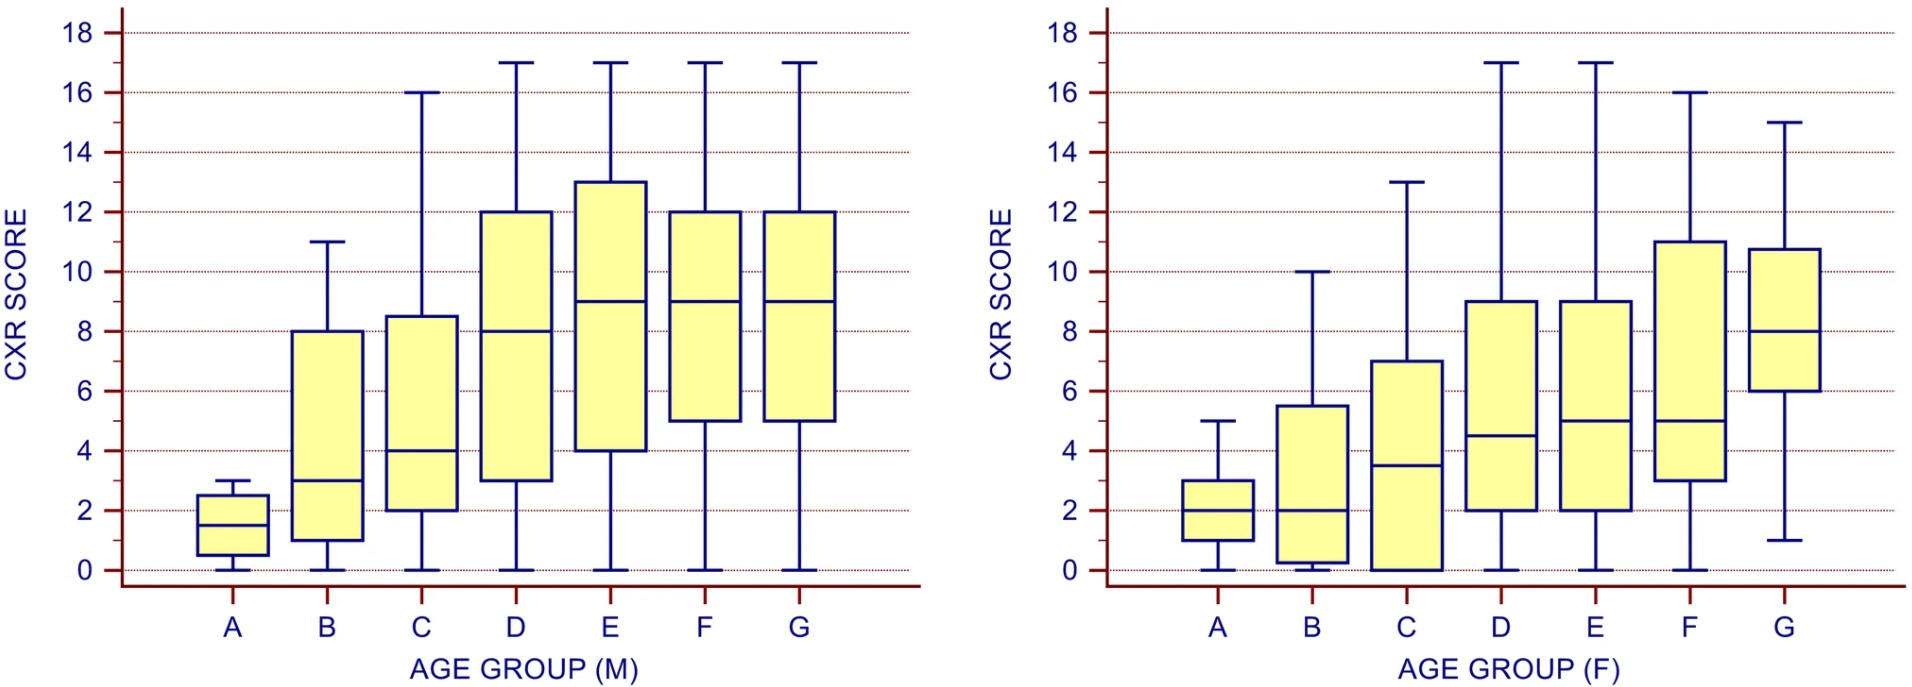
\includegraphics[width=15cm]{age-sex.jpg}
\caption{Rozkład wyników badania RTG klatki piersiowej (CXR) w zależności od grupy wiekowej u mężczyzn (M) i kobiet (F)}
\end{figure}

Podsumowując, autorzy badania wskazują na istotny wpływ wieku na śmiertelność przy infekcji COVID-19. Stwierdzono, że mężczyźni w wieku 50 lat lub starsi i kobiety w wieku 80 lat lub starsze wykazywali najwyższe ryzyko rozwoju ciężkiej choroby płuc. \cite{wang2020}

\subsection{Zmienne meteorologiczne jako determinanty częstotliwości zachorowań na COVID-19}

Opublikowany w wrześniu 2020 artykuł \emph{Effect of meteorological factors on COVID-19 cases in Bangladesh} koncertuje się na opisie wpływu warunków pogodowych na możliwość zarażenia się koronawirusem. Badanie na temat którego powstał wspomniany artykuł przeprowadzono na terytorium Bangladeszu. Kraj znajduję się w strefie klimatu zwrotnikowego, a na jego terytorium występują 3 główne pory roku: pre-monsun,monsun, post-mosum. Ze względu na złożone warunki klimatyczne i dużą gęstość zaludnienia obszar ten jest uznawany za wysoce wrażliwy na zmiany klimatu.


Badanie jest również wartościowe ze względu na możliwość powiązania poziomu ryzyka zachorowania na COVID-19 z samym przebiegiem choroby. Takie założenie znalazło potwierdzenie w 2 opracowanych już badaniach. W pierwszym z nich,  badaniu \emph{Virological assessment of hospitalized patients with COVID-2019} podjęto się opisania przebiegu zachorowania z punktu widzenia rodzaju jak i natężenia cząsteczek wirusa.\cite{wolfel2020} Jednocześnie w badaniu \emph{SARS-CoV-2 concentrations and virus-laden aerosol size distributions in outdoor air in north and south of Italy} stwierdzono fakt o wysokim znaczeniu stężenia wirusa i częstości zachorowań. \cite{chirizzi2020}

Do przeprowadzenia badania zebrano dane z 43 stacji meteorologicznych z których wyodrębniono informacje na temat kilkunastu parametrów atmosferycznych (maksymalna temperatura dobowa (MaxT), minimalna temperatura dobowa (MinT), siła wiatru (WS), wilgotność relatywna (RH), wilgotność absolutna (AH) itp.) dla odpowiadającym im regionów. Na podstawie danych o przypadkach zachorowani na COVID-19 z odpowiadających im obszarów ustalono wskaźnik relatywnego ryzyka (RR), który oceniał prawdopodobieństwo zarażenia się SARS-CoV-2 w określonym dniu. Ze względu na od 2 do 14 dniowy okres inkubacji wirusa przyjęto maksymalnie 14 dniowe opóźnienie między obserwacjami meteorologicznymi, a poszczególnymi przypadkami zgłoszonych zachorowań.

Koherencja transformaty falkowej (WTC) i częściowa koherencja falkowa (PWC) zostały wykorzystane w tym badaniu do uzyskania wyrazów rozdzielczości czasowej i częstotliwościowej zmiennych klimatycznych i przypadków COVID-19 w Bangladeszu. WTC kwantyfikuje wielkość kowariancji między dwoma szeregami czasowymi, która waha się od 0 do 1 (0 $\leq$ R2 $\leq$ 1). 0 odnosi się do całkowitego braku spójności, podczas gdy 1 odnosi się do doskonałej spójności. Zakres ten definiuje się jako kwadrat widma krzyżowego znormalizowanego przez wygładzone indywidualne widmo mocy. 

RH wykazało silny pozytywny znaczący związek z przypadkami COVID-19 w Singapurze. Oznacza to, że maksymalne RH (71,4 $\pm$ 4\%) w maju sprzyjało rozprzestrzenianiu się COVID-19. WS wykazał znaczący związek z potwierdzonymi przypadkami COVID-19 w Bangladeszu. Natomiast AP wykazywał stosunkowo silną odwrotną zależność z pozytywnymi przypadkami zakażenia COVID-19 w Bangladeszu w początkowej fazie epidemii SARS-CoV-2. Ogólnie rzecz biorąc, wysokie wartości MinT, RH i AH wraz z niskimi WS w maju nasiliły rozprzestrzenianie się SARS-CoV-2.

Przedstawiono zależność opóźnionej odpowiedzi RR na wzrost o 1 jednostkę wszystkich wskaźników meteorologicznych w różnych dniach opóźnienia (do 14 dni). Największe RR dla MaxT wyniosło 1,00 (95\% CI 0,99-1,01) w opóźnieniu 6-dniowym, a najmniejsze 0,92 (95\% CI 0,88-0,95) bez opóźnienia. Największe RR dla MinT wyniosło 1,04 (95\% CI 1,01-1,06) w opóźnieniu 11-dniowym, a najmniejsze 1,01 (95\% CI 0,99-1,02) w opóźnieniu 2-dniowym. 

\begin{figure}[H]
\centering
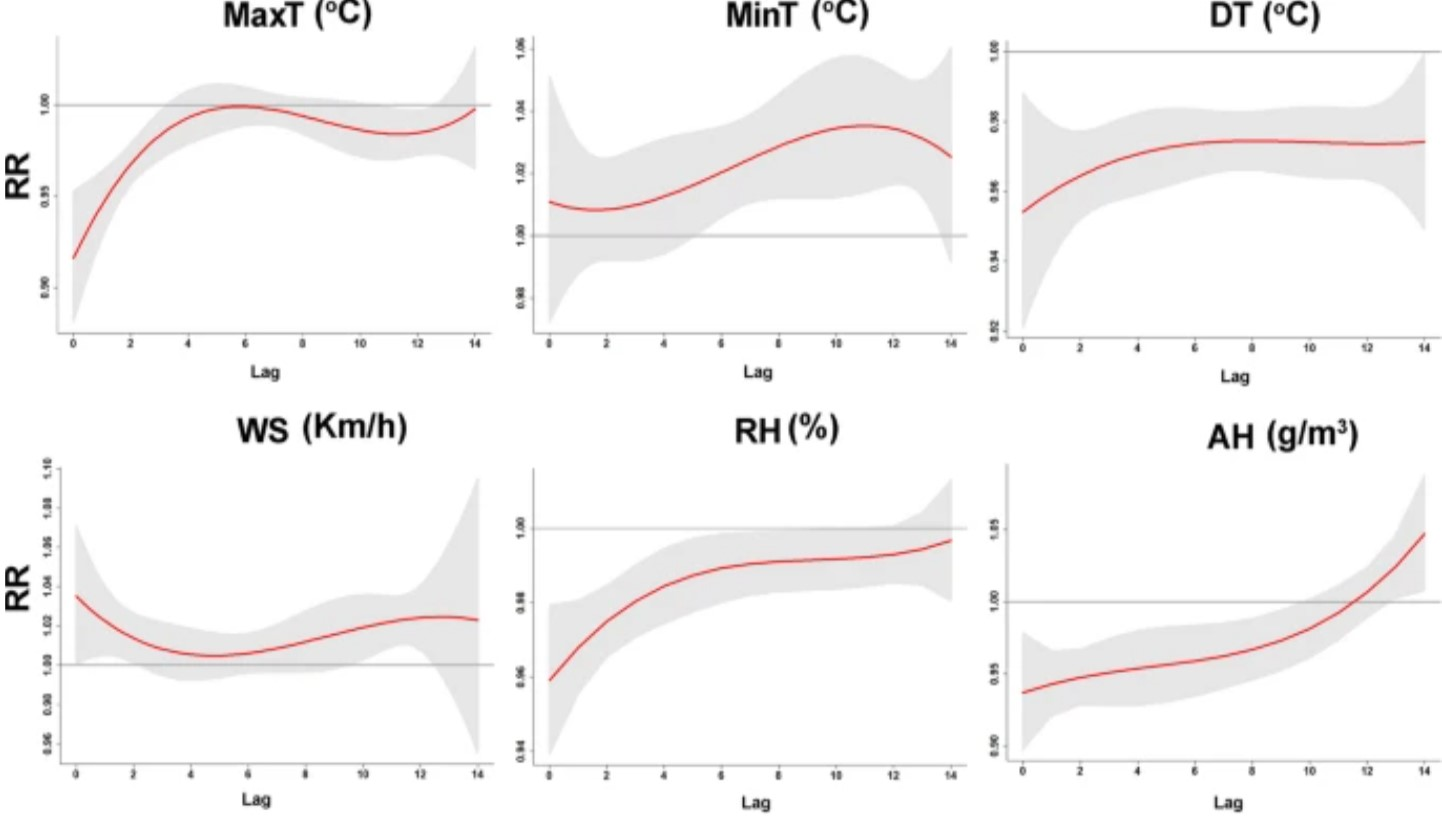
\includegraphics[width=15cm]{clmate-factors.jpg}
\caption{Pojedyncze efekty MaxT, MinT, DT, WS, RH i AH. Laboratorium Y oznacza wartość ryzyka względnego (RR)}
\end{figure}

Podsumowując, zaobserwowano znaczący wpływ pomiędzy nasileniem COVID-19 a zmiennymi meteorologicznymi. Temperatura, może odgrywać istotną rolę w procesach życiowych człowieka oraz w zakresie ograniczania i kontroli epidemii. Ponadto, oddnotowano wpływ siły wiatru na propagowanie epidemii. Wiatr może wpływać na czas zawieszenia koronawirusa i jego rozprzestrzenianie się. Badanie wykazało, że wskaźnik RR wyraźnie wzrósł, w czasie gdy WS podwyższył się o ponad 21 km/h. Stężenie koronawirusa może być rozrzedzone przez podwyższony WS, co może stanowić prawdopodobne wyjaśnienie tego wyniku. Można wnioskować, iż temperatura i prędkość wiatru wykazują silny związek z rozpoczęciem i przebiegiem choroby COVID-19 w Bangladeszu. \cite{hasanuzzaman2020}



% --- chapter ---------------------------------------------------------
\clearpage
\section{Opis zbioru danych}
\label{chapter:data-set}

%- liczebność oraz źródło zbioru danych \\
%- opisy zmiennych \\
%- rozkład zmiennych \\
%- charakterystyki zmiennych (np. średnie, odchylenia std ) \\
%- charakterystyka brakujących danych \\
%- problemy wynikające z brakujących danych

Do przeprowadzenia badania zostały użyte 3 zbiory danych: 
\begin{itemize}
  \item dane na temat poszczególnych przypadków zachorowań na COVID-19 w USA - pochodzą z zasobów Centers for Disease Control and Prevention
  \item wskaźniki atmosferyczne dla poszczególnych części USA - pochodzą z zasobów National Centers for Environmental Information
  \item dane demograficzne  dla poszczególnych części USA - pochodzą z portalu ArcGis
\end{itemize}



\subsection{Zbiór danych dotyczący poszczególnych przypadków zachorowań na COVID-19}


Zbiór danych pochodzi z zastrzeżonych zasobów Centers for Disease Control and Prevention (CDC). Zbiór ten został udostępniony po bezpośredniej prośbie skierowanej do jego właścicieli i za ich pozwoleniem został wykorzystany w tej pracy. Zebrane są w nim podstawowe dane medyczne osób ze stwierdzonym COVID-19 zarejestrowanych przez amerykańską służbę zdrowia z okresu od pierwszego potwierdzonego przypadku zachorowania (styczeń 2020) do końca lutego 2021 roku - łącznie 20,5 mln obserwacji. Zmienne, które zostały użyte w tej pracy zostały scharakteryzowane w tabeli \ref{table:zmienneCDC} .

\begin{table}[H]
  \centering
\resizebox{15cm}{!}{
\centering
\csvautotabular[respect underscore=true]{tables/zmienne_CDC.csv}
}
\caption{Zmienne ze zbioru CDC użyte w dalszej części pracy.}
\label{table:zmienneCDC}
\end{table}

W zbiorze danych występują 3 typy brakujących danych. Najczęściej występującym jest \emph{Unknown} i jak autor zbioru danych opisuje kodowany był w przypadku udzielenia dokładnie takiej odpowiedzi do pytania szpitalnej ankiety. Kolejnym typem jest  \emph{Missing} i występuję w przypadkach nie udzielenia jakiejkolwiek odpowiedzi. Najrzadziej występującym typem wskazującym brak danych jest \emph{NaN} i zakodowany został w miejscach logicznej nieścisłości danych oraz w przypadkach błędów na poziomie zapisu danych w centralnej bazie.

Pomimo bardzo dużej ilości obserwacji wadą zbioru okazał się niski udział w pełni opisanych przypadków (większość zmiennych zawiera mniej niż 25\% uzupełnionych danych). Obliczone częstości występowania oraz korelacje brakujących danych pomiędzy zmiennymi z uwzględnieniem oraz bez uwzględnienia typów braków danych nie wskazała przyczyny dużego natężenia braku danych. Uznano również, że lokalizacja brakujących danych jest niedeterministyczna. Ze względu na jakościową naturę zmiennych oraz wysoki udział brakujących danych nie możliwe było przeprowadzenie imputacji brakujących danych. Znikoma wartość informacja niesiona przez brak danych przyczyniłaby się do zaburzenia interpretacji wyników dalszej części pracy dlatego podjęto decyzję o odrzuceniu wszystkich niepełnych obserwacji. Dalsza część pracy odnosi się do wyselekcjonowanych tym sposobem 171 147 pełnych obserwacji. 

W zbiorze udostępnionym przez CDC pacjenci zostali podzieleni na 8 grup wiekowych o rozpiętości 10 lat, a dla najstarszych stworzono grupę 80+. Zmienna \emph{race\_ethnicity\_combined} przyjmuje wartości: \emph{American Indian/Alaska Native, Non-Hispanic} dla natywnych mieszkańców Ameryki Północnej, \emph{Asian, Non-Hispanic} dla rasy żółtej, \emph{Black, Non-Hispanic} dla rasy czarnej, \emph{Hispanic/Latino} dla mniejszości latynoskiej, \emph{Native Hawaiian/Other Pacific Islander, Non-Hispanic} dla natywnych mieszkańców wysp Pacyfiku, \emph{White, Non-Hispanic} dla rasy białej oraz \emph{Multiple/Other, Non-Hispanic} dla pozostałych. Wartości zmiennej \emph{sex} zostały przekodowane na 1 dla mężczyzn oraz 0 dla kobiet. Wartości dla pozostałych zmiennych dwumianowych zostały przekodowane na 1 dla wartości \emph{Yes} oraz na 0 dla \emph{No}.

Najliczniejszą grupą w zbiorze okazali się być przedstawiciele rasy białej i składają się na 73.8\% wszystkich obserwacji. Natywni mieszkańcy wysp Pacyfiku (0,38\%) oraz natywni mieszkańcy Ameryki Północnej (0,11\%) stanowią najmniej liczne grupy etniczne w opisywanym zbiorze danych. Udział procentowy kobiet jest porównywalny do udziału mężczyzn i wynosi odpowiednio 44,2\% dla mężczyzn oraz 55,8\% dla kobiet (Wykres: \ref{figure:sex-race-count})

\begin{figure}[H]
\centering
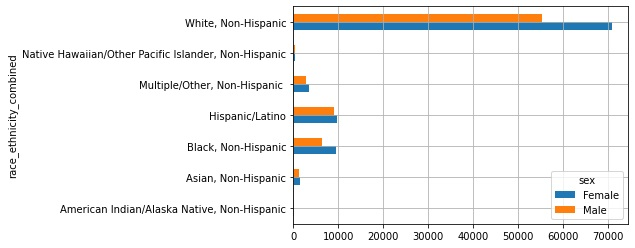
\includegraphics[width=15cm]{race_sex_count_plot.jpg}
\caption{Liczebność poszczególnych grup etniczno-rasowych z podziałem na płeć}
\label{figure:sex-race-count}
\end{figure}

Najczęstszymi symptomami COVID-19 był kaszel (60,9\%), ból głowy (59,0\%) oraz bóle mięśniowe (53.1\%). Najrzadziej pacjenci informowali o dolegliwościach związanych z bólem brzucha (11,5\%) oraz nudnościami (21,5\%) W opisanym zbiorze wskaźnik hospitalizacji wyniósł 6,72\%, a wskaźnik śmiertelności 1,28\%.

\begin{figure}[H]
\centering
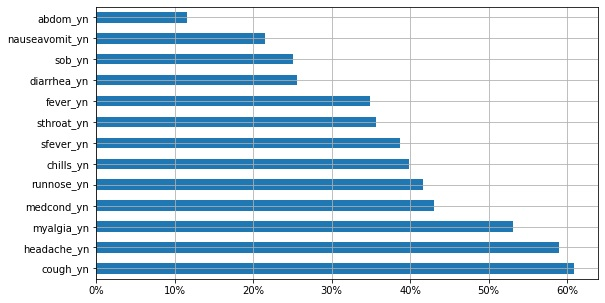
\includegraphics[width=15cm]{symptoms-freq.jpg}
\caption{Częstość występowania poszczególnych objawów COVID-19}
\end{figure}



\subsection{Zbiory danych zawierający wskaźniki atmosferyczne dla poszczególnych części USA}

Kolejne zbiory danych jakie użyto w tej pracy pochodzą z upublicznionych zasobów National Centers For Environmental Information. Zawierają one dane na temat najważniejszych parametrów metrologicznych obserwowanych przez największe miasta USA. Udostępnione dane zawierają średnie wartości zagregowane na poziomie miesięcznym i rocznym. Korzystając z tego źródła do tej pracy użyto trzech poniższych tabel:
\begin{itemize}
  \item \emph{Normal Daily Maximum Temperature, °F} - średnie dobowe temperatury obliczone na podstawie obserwacji zebranych w latach 1971-2000 wyrażone w stopniach Fahrenheita.
  \item \emph{Wind - Average Speed (MPH)} - średnie prędkości wiatru obliczone bez uwzględnienia jego kierunku wyrażone w milach na godzinę.
  \item \emph{Average Relative Humidity (Percent) - Morning (M) and Afternoon (A)} - średnie wilgotności powietrza rano i wieczorem obliczone wyrażone w procentach.
\end{itemize}

Ze względu na fakt, iż dla niektórych hrabstw nie odnotowano żadnych obserwacji postanowiono zgrupować dane na poziomie stanów i wyliczyć dla nich średnie wartości. W zestawieniu rocznym najgorętszym stanem okazała się Floryda osiągając średnią temperaturę 72,1 \textdegree F (22,3 \textdegree C), najchłodniejszym zaś Alaska ze średnią temperaturą 32,8 \textdegree F (0,4 \textdegree C). Największa średnia roczna prędkość wiatru przypada na stan Kansas (11,2 mph) i Massachusetts (10,9 mph), najmniejsza zaś w stanie West Virginia (5,6 mph). 

\begin{figure}[H]
\centering
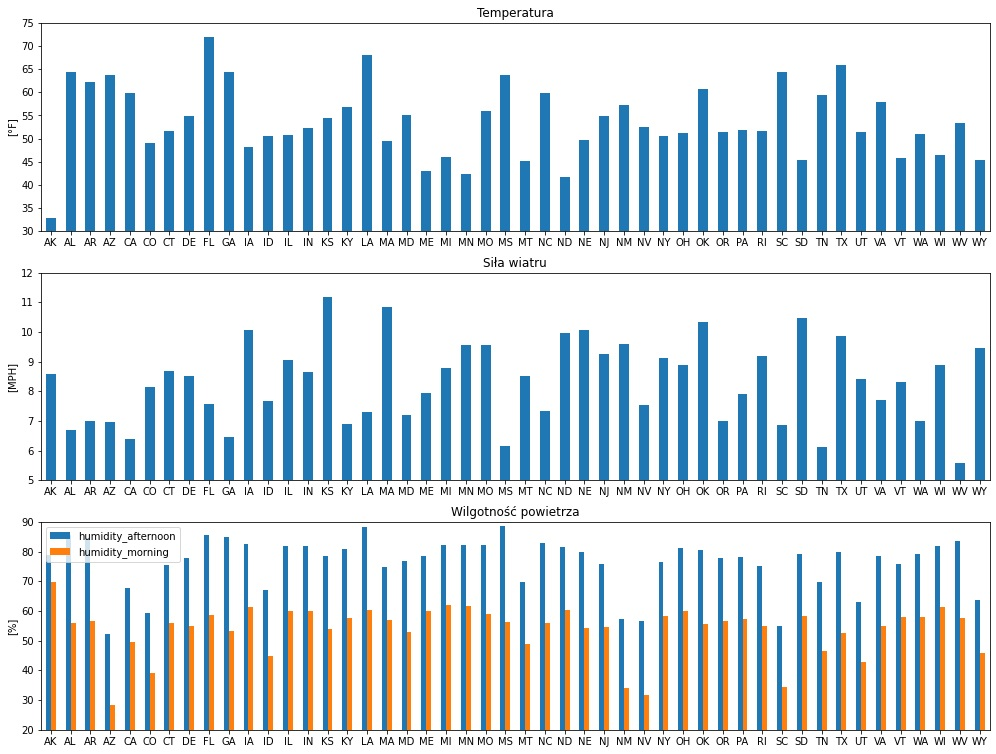
\includegraphics[width=15cm]{atm-all.jpg}
\caption{Wybrane wskaźniki atmosferyczne zagregowane na poziomie rocznym zgrupowane dla poszczególnych stanów. }
\end{figure}


\subsection{Zbiór danych zawierający dane demograficzne}

Ostatnim zbiorem jaki został wykorzystany w tej pracy jest zbiór \emph{USA Counties} pochodzący z ArcGIS Hub. Autorem zbioru jest ArcGIS Data and Maps (poprzednio Esri Data \& Maps), czyli sam zespół portalu ArcGIS. Oprócz danych demograficznych w zbiorze znaleźć można dane geograficzne oraz wskaźniki związane z rolnictwem. Dane demograficzne datowane są na 2010 rok i pochodzą z amerykańskiego spisu powszechnego. Wszystkie zmienne zostały określone na poziomie hrabstw.

Ze względu na tematykę pracy postanowiono wykorzystać z opisanego zbioru tylko jedną zmienną, czyli \emph{POP\_SQMI} - zagęszczenie ludności na mile kwadratową. Analiza zbioru wykazała, że najmniej rzadziej zaludnione hrabstwa w USA to Lake and Peninsula, North Slope, Denali, Yakutat oraz Loving z gęstością zaludnienia na poziomie 0,1 osoby na mile kwadratowej. Wszystkie wymienione hrabstwa oprócz Loving (stan Texas) zlokalizowane są na obszarze Alaski. Najgęściej zaludnione hrabstwa to New York (73032,2 osoby na mile kwadratową), Kings (38512,3 osoby na mile kwadratową) oraz Bronx (34919,1 osoby na mile kwadratową) - wszystkie zlokalizowane w stanie New York. Gęstość zaludnienia Stanów Zjednoczonych, obliczona przez zsumowanie populacji wszystkich hrabstw i podzielenie przez sumę ich powierzchni, wynosi 91,1 osoby na mile kwadratową.

\begin{figure}[H]
\centering
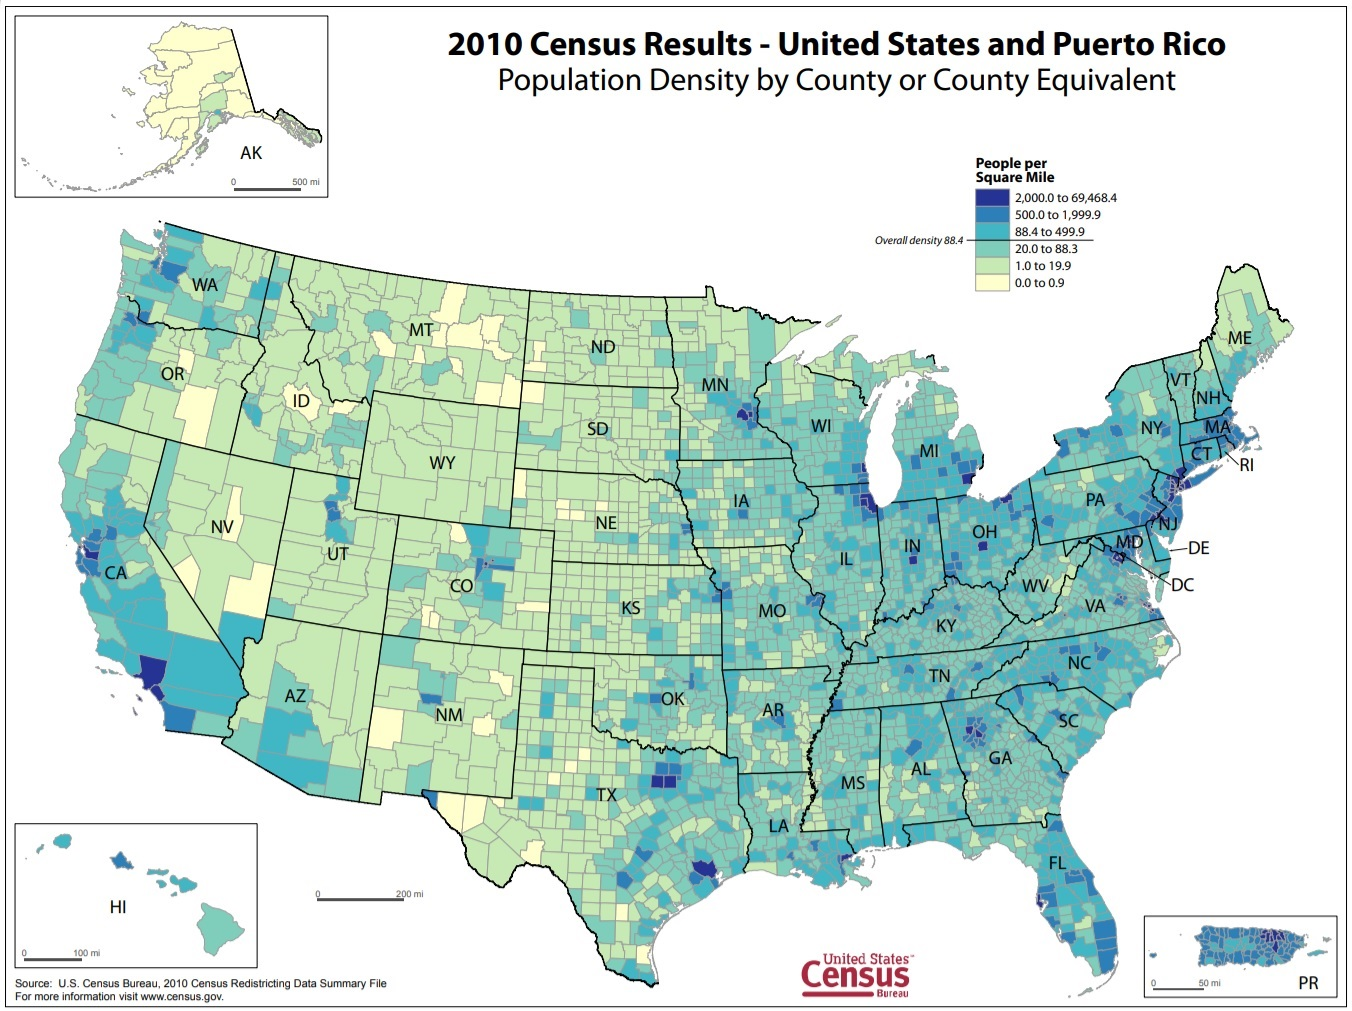
\includegraphics[width=15cm]{us-desity.jpg}
\caption{Zagęszczenie ludności zwizualizowane na mapie Stanów Zjednoczonych. }
\end{figure}

\subsection{Docelowy zbiór danych}

Po uzyskaniu zbiorów z zewnętrznych zasobów oraz wstępnego oczyszczenia danych postanowiono stworzyć zbiór danych, który posłuży do budowy modelu XGBoost. Podstawą do budowy tego zasobu był zbiór danych związany z poszczególnymi obserwacjami zachorowań COVID-19 do którego dowiązano w określony sposób pozostałe zbiory zbiory.

Pierwszym krokiem było dowiązanie wskaźników atmosferycznych do zbioru danych związanego z obserwacjami COVID-19 . Dokonano tego przez zmapowanie miesiąca zachorowania i zamieszkanego stanu ze wskazaną zmienną meteorologiczną przypisaną dla tego stanu w tym terminie. W ten sposób otrzymano następujące zmienne:
\begin{itemize}
  \item \emph{avg\_temp} - średnia dobowa temperatura wyrażona w stopniach Fahrenheita.
  \item \emph{avg\_wind} - średnia prędkość wiatru wyrażona w milach na godzinę.
  \item \emph{avg\_humidity\_M} - średnia wilgotność powietrza rano wyrażona w procentach.
  \item \emph{avg\_humidity\_A} - średnia wilgotność powietrza wieczorem wyrażona w procentach.
\end{itemize}

Kolejnym etapem było dowiązanie powstałego w poprzednim kroku zbioru ze zbiorem danych uzyskanym z portalu ArcGIS. Osiągnięto to przez zmapowanie nazwy zamieszkanego hrabstwa osoby ze stwierdzonym COVID-19 z gęstością zaludnienia w tym obszarze. W ten sposób uzyskano zmienną \emph{pop\_density}, która określa gęstość zaludnienia wyrażoną w liczbie osób na mile kwadratową.

Ostatnim krokiem było odrzucenie niepożądanych zmiennych z powstałego zbioru danych. Ten etap był konieczny gdyż niektóre zmienne nie miały bezpośredniego związku z wyjaśnieniem przedmiotu tej pracy. Odrzuconymi zmiennymi były:  \emph{county\_fips\_code},  \emph{res\_county}, \emph{res\_state}, \emph{cdc\_case\_earliest\_dt} oraz \emph{date\_month}.


\begin{table}[H]
  \centering
\resizebox{15cm}{!}{
\centering
\csvautotabular[respect underscore=true]{tables/zmienne_ostateczne.csv}
}
\caption{Opis zmiennych w finalnym zbiorze danych}
\label{table:zmienne-finalne}
\end{table}

% --- chapter ---------------------------------------------------------
\clearpage
\section{Metody}

%- opis kolejności obliczeń/transformacji/budowy modelu \\
%- opis użytego modelu (docelowo: xgboost) oraz jego zasadność względem niezbalansowanej próby\\
%- opis metod walidacji oraz jakości modelu (F1-score, accuracy) \\
%- opis sposobu interpretacji wpływu zmiennych objaśniających na zmienną objaśnianą (docelowo: SHAP)

\subsection{Podział zbioru na treningowy, walidacyjny i testowy}
\label{chapter:train-test-split}
W uczeniu maszynowym powszechnym zadaniem jest badanie i konstruowanie algorytmów, które potrafią uczyć się na podstawie danych i dokonywać predykcji na ich podstawie. \cite{kohavi1998} Model jest początkowo dopasowywany do zbioru danych treningowych, który jest zbiorem przykładów używanych do dopasowania parametrów (np. wag połączeń między neuronami w sztucznych sieciach neuronowych) modelu. Model (np. sieć neuronowa lub naiwny klasyfikator Bayesa) jest trenowany na zbiorze danych treningowych za pomocą metody uczenia nadzorowanego, na przykład za pomocą metod optymalizacji, takich jak opadanie gradientowe lub stochastyczne opadanie gradientowe. W praktyce, zbiór danych szkoleniowych często składa się z par wektora wejściowego (lub skalara) i odpowiadającego mu wektora wyjściowego (lub skalara), gdzie klucz odpowiedzi jest powszechnie oznaczany jako cel (lub etykieta). Bieżący model jest uruchamiany z zestawem danych treningowych i wytwarza wynik, który jest następnie porównywany z celem, dla każdego wektora wejściowego w zestawie danych treningowych. W oparciu o wynik porównania i określony algorytm uczenia się, parametry modelu są dostosowywane. Dopasowanie modelu może obejmować zarówno selekcję zmiennych, jak i estymację parametrów.

Następnie, dopasowany model jest używany do przewidywania odpowiedzi dla obserwacji w drugim zbiorze danych zwanym zbiorem danych walidacyjnych. Zbiór danych walidacyjnych zapewnia bezstronną ocenę dopasowania modelu na zbiorze danych treningowych podczas dostrajania hiperparametrów modelu (np. liczba jednostek ukrytych - warstw i szerokości warstw - w sieci neuronowej). Walidacyjne zbiory danych mogą być użyte do regularyzacji poprzez wczesne zatrzymanie (zatrzymanie treningu, gdy błąd na walidacyjnym zbiorze danych wzrasta, ponieważ jest to oznaką przepasowania do zbioru treningowego). Ta prosta procedura jest skomplikowana w praktyce przez fakt, że błąd zbioru walidacyjnego może wahać się podczas treningu, tworząc wiele lokalnych minimów. Ta komplikacja doprowadziła do powstania wielu reguł ad hoc służących do określania, kiedy przepełnienie naprawdę się rozpoczęło.

Finalnie, testowy zbiór danych jest zbiorem danych używanym w celu zapewnienia bezstronnej oceny ostatecznego dopasowania modelu na treningowym zbiorze danych. Jeśli dane w testowym zbiorze danych nigdy nie były używane w trenowaniu modelu (na przykład w walidacji krzyżowej), testowy zbiór danych jest również nazywany zbiorem danych przejściowych (ang. holdout dataset). Termin \emph{zbiór walidacyjny} jest czasami używany zamiast terminu \emph{zbiór testowy} (np. jeżeli oryginalny zbiór danych został podzielony tylko na dwa podzbiory, zbiór testowy może być określany jako zbiór walidacyjny).\cite{brownlee2017}

Docelowy zbiór danych użyty w tej pracy został losowo podzielony na treningowy, walidacyjny i testowy w stosunku 3:1:1. Etap ten umożliwił w kolejnych krokach dobranie właściwych parametrów oraz zbudowanie optymalnego modelu.

\subsection{Budowa modelu klasyfikacyjnego XGBoost}

XGBoost to biblioteka oparta na licencji otwartego kodu źródłowego, która dostarcza regularyzujący framework do wspomagania gradientowego dla C++, Javy, Pythona, R, Julii, Perla i Scali. XGBoost jest kompatybilny z systemami Linux, Windows i macOS. Działa na pojedynczej maszynie, jak również na frameworkach przetwarzania rozproszonego Apache Hadoop, Apache Spark i Apache Flink. 

Klasyfikator XGBoost posiada wiele hiperparametrów, które mogłyby posłużyć do strojenia modelu. Najwrażliwsze z nich zostały iteracyjnie wybrane do stworzenia optymalnego modelu dla tej pracy. Pozostałe, mający niski wpływ, przyjęły domyślne wartości zalecone przez autorów biblioteki. Iteracyjnie dopasowywane hiperparametry to:
\begin{itemize}
 \item \emph{learning\_rate} - Tempo uczenia modelu. Zmniejszanie wielkości kroków w aktualizacji zapobiega przeszacowaniu modelu.
 \item \emph{max\_depth} - Maksymalna głębokość drzewa. Zwiększenie tej wartości sprawi, że model będzie bardziej złożony i prawdopodobnie obszerniejszy.
 \item \emph{min\_child\_weight} - Minimalna suma wagi instancji w poprzedniku. Jeśli krok podziału drzewa skutkuje powstaniem węzła liścia z sumą wagi instancji mniejszą niż min\_child\_weight, wówczas proces tworzenia rezygnuje z dalszego podziału. 
 \item \emph{scale\_pos\_weight} - Współczynnik zbalansowania zbioru treningowego. Kontrola równowagi wag dodatnich i ujemnych, przydatna w przypadku niezrównoważonych klas.
 \item \emph{gamma} - Minimalna redukcja strat wymagana do utworzenia kolejnej partycji na węźle liścia drzewa. Im większa wartość gamma, tym bardziej konserwatywny algorytm.
\end{itemize}

By zapewnić wysoką wydajność procesowania autorzy biblioteki zaparzyli ją w wysoce wydajne mechanizmy. Biblioteka XGBoost obsługuję między innymi trzy formy wspomagania gradientowego:
\begin{itemize}
  \item Algorytm Gradient Boosting zwany również maszyną gradient boostingową z uwzględnieniem współczynnika uczenia.
  \item Stochastyczny Gradient Boosting z podpróbkowaniem na poziomie wiersza, kolumny i kolumny na poziom rozdzielenia.
  \item Regularyzowany Gradient Boosting z regularyzacją zarówno L1 jak i L2.
\end{itemize}

Implementacja algorytmu została zaprojektowana pod kątem efektywności czasu obliczeń i zasobów pamięci. Niektóre kluczowe cechy implementacji algorytmu obejmują:
\begin{itemize}
 \item Implementacja uwzględniająca rzadkość danych z automatyczną obsługą brakujących wartości danych.
 \item Struktura blokowa wspierająca paralelizację konstrukcji drzewa.
 \item Inkrementalne trenowanie modelu, dzięki któremu można dalej wzmacniać już dopasowany model na nowych danych.
\end{itemize}

Oprócz poprzednio wymienionych mechanizmów algorytm klasyfikatora XGBoost umożliwia korzystanie z niezbalansowanych zbiorów danych. Dla użytkownika klasyfikatora ta funcjonalność udostępniona jest przez hiperparametr \emph{scale\_pos\_weight}. Ze względu na niezbalansowany zbiór wykorzystany w tej pracy (zmienna objaśniana \emph{death\_yn} zawiera tylko 1,3\% pozytywnych wartości) mechanizm ten okazał się niezbędny. Jest to rzadko spotykana funkcjonalność zaimplementowana w modelach uczenia maszynowego. Ze względu na ten opisany mechanizm, wysoką wydajność obliczeń i zasobów oraz dużą popularność w komercjalnych zastosowaniach klasyfikator XGBoost został wybrany na docelowy model uczenia maszynowego dla tej pracy. 

\subsection{Interpretacja wskaźników jakości modelu}

\subsubsection{F1-score}

W analizie statystycznej klasyfikacji binarnej, F1-score lub F1-measure jest miarą dokładności testu. Jest on obliczany na podstawie miary precyzji (ang. precision) i czułości (ang. recall), gdzie precyzja jest liczbą prawdziwie pozytywnych wyników podzielonych przez liczbę wszystkich pozytywnych wyników, w tym tych, które nie zostały prawidłowo zidentyfikowane, a czułość jest liczbą prawdziwie pozytywnych wyników podzielonych przez liczbę wszystkich próbek, które powinny być zidentyfikowane jako pozytywne. Precyzja jest również znana jako pozytywna wartość predykcyjna, a wycofanie jest również znane jako czułość w diagnostycznej klasyfikacji binarnej. Wynik F1-score jest średnią harmoniczną precyzji i czułości. 

Najwyższą możliwą wartością F1-score jest 1.0, wskazując idealną precyzję i czułość, a najniższą możliwą wartością jest 0, jeśli precyzja lub czułość wynosi zero. Wynik F1-score jest również znany jako współczynnik Sørensena-Dice'a lub współczynnik podobieństwa Dice'a (DSC).

\[ F_1 = \frac{2}{recall^{-1} + precision^{-1}} = 2 * \frac{precision * recall}{precision + recall} \]

F1-score został użyty do wyznaczenia najlepszych hiperparametrów. Po podstawieniu kolejnych kombinacji hiperparametrów do budowanego modelu dla danych treningowych obliczana była wartość F1-score. Za najlepsze hiperparametry uznano te dla, których model przetestowany na danych walidacyjnych osiągnął najwyższą wartość F1-score.\cite{tharwat2018}

Ze względu na szerokie spektrum własności oraz celność tego wskaźnika F1-score został użyty również do przedstawienia jakości docelowego modelu. Wykonano to przez przetestowanie modelu na danych testowych i późniejszym obliczeniu wartości F1-score.\cite{powers2011}

\subsubsection{Dokładność}

W przypadku zadań klasyfikacyjnych terminy \emph{prawdziwie dodatni (tp)}, \emph{prawdziwie ujemny (tn)}, \emph{fałszywie dodatni (fp)} i \emph{fałszywie ujemny (fn)} porównują wyniki testowanego klasyfikatora z wiarygodną oceną zewnętrzną. Terminy pozytywny i negatywny odnoszą się do przewidywań klasyfikatora (czasami znanych jako oczekiwania), a terminy prawdziwy i fałszywy odnoszą się do tego, czy przewidywania te odpowiadają zewnętrznemu osądowi (czasami nazywanemu jako obserwacja). \cite{fawcett2005}

Dokładność (ang. accuracy) jest używana jako statystyczna miara tego, jak dobrze binarny test klasyfikacyjny prawidłowo identyfikuje lub wyklucza stan. Oznacza to, że dokładność jest proporcją prawidłowych przewidywań (zarówno prawdziwie pozytywnych, jak i prawdziwie negatywnych) wśród całkowitej liczby badanych przypadków. Jako takie, porównuje ono szacunki prawdopodobieństwa przed i po teście. Aby kontekst był jasny dzięki semantyce, jest ona często określana jako \emph{Rand accuracy} lub \emph{Rand index}. Jest to parametr testu.\cite{powers2015} Poniżej wzór dokładności:
\[ Accuracy = \frac{tp + tn}{tp + tn + fp + fn} \]

Miara dokładności sprawdza się przede wszystkim w zbalansowych zbiorach. Ze względu na niską liczbę pozytywnych wartości zmiennej objaśnianej \emph{death\_yn} miara ta posłużyła wyłącznie do opisu docelowego modelu.\cite{tharwat2018}

\subsubsection{Tablica pomyłek}

W dziedzinie uczenia maszynowego, a konkretnie w problematyce klasyfikacji statystycznej, macierz pomyłek, zwana też macierzą błędów, jest specyficznym układem tabelarycznym pozwalającym na wizualizację działania algorytmu, zazwyczaj uczenia nadzorowanego (w uczeniu nienadzorowanym nazywana jest zwykle macierzą dopasowania). Każdy wiersz macierzy reprezentuje instancje w klasie rzeczywistej, natomiast każda kolumna reprezentuje instancje w klasie przewidywanej, lub odwrotnie - oba warianty są spotykane w literaturze. Nazwa macierzy pochodzi stąd, że pozwala ona łatwo zorientować się, czy system nie myli dwóch klas (tj. powszechnie błędnie przypisuje jedną klasę do drugiej).

Jest to specjalny rodzaj tabeli kontyngencji, z dwoma wymiarami (\emph{rzeczywisty} i \emph{przewidywany}) oraz identycznymi zestawami \emph{klas} w obu wymiarach (każda kombinacja wymiaru i klasy jest zmienną w tabeli kontyngencji). \cite{powers2011}

Oprócz wizualnego przedstawienia jakości modelu tablica pomyłek może również posłużyć do obliczenia innych wskaźników takich jak czułość czy swoistość. Ze względu na zaprezentowane właściwości macierz błędów została użyta do opisu docelowego modelu.

\subsubsection{Krzywa ROC}

Krzywa charakterystyki odbiornika (ang. receiver operating characteristic curve, ROC curve) jest wykresem, który ilustruje zdolność diagnostyczną systemu klasyfikatora binarnego w miarę zmiany progu dyskryminacji. Metoda ta została pierwotnie opracowana dla operatorów wojskowych odbiorników radarowych począwszy od 1941 roku, co doprowadziło do jej nazwy.

Krzywa ROC jest tworzona poprzez wykreślenie współczynnika prawdziwych pozytywów (TPR) względem współczynnika fałszywych pozytywów (FPR) przy różnych ustawieniach progu. Współczynnik prawdziwych pozytywów jest również znany jako czułość, wycofanie lub prawdopodobieństwo wykrycia w uczeniu maszynowym. Współczynnik fałszywych wyników jest również znany jako prawdopodobieństwo fałszywego wyniku i może być obliczany jako (1 - specyficzność). Można o niej również myśleć jako o wykresie mocy jako funkcji błędu typu I reguły decyzyjnej (gdy wydajność jest obliczana tylko na podstawie próbki populacji, można o niej myśleć jako o estymatorze tych wielkości). Krzywa ROC jest więc czułością lub wycofaniem w funkcji błędu. Ogólnie rzecz biorąc, jeśli znane są rozkłady prawdopodobieństwa zarówno dla wykrywania, jak i fałszywego wyniku, krzywą ROC można wygenerować, wykreślając funkcję rozkładu kumulatywnego (obszar pod rozkładem prawdopodobieństwa od do progu dyskryminacji) prawdopodobieństwa wykrywania na osi y versus funkcję rozkładu kumulatywnego prawdopodobieństwa fałszywego wyniku na osi x.

Analiza ROC dostarcza narzędzi do wyboru możliwie optymalnych modeli i odrzucania modeli suboptymalnych niezależnie od (i przed określeniem) kontekstu kosztów lub rozkładu klasy. Analiza ROC jest w bezpośredni i naturalny sposób związana z analizą kosztów i korzyści przy podejmowaniu decyzji diagnostycznych.\cite{fawcett2005}

Jeśli poprawnie używane, krzywe ROC są bardzo potężnym narzędziem jako statystyczna miara wydajności w teorii wykrywania/klasyfikacji i testowaniu hipotez, ponieważ pozwalają na posiadanie wszystkich istotnych wielkości w jednym wykresie. Ze względu na te właściwości krzywa ROC została użyta do przedstawienia jakości docelowego modelu stworzonego dla tej pracy.

\subsection{Interpretacja wyników modelu przez wartości SHAP}

SHAP (SHapley Additive exPlanations) jest podejściem opartym na teorii gier, służącym do wyjaśniania wyników dowolnego modelu uczenia maszynowego. Interpretując model wytrenowany na zbiorze cech jako funkcję wartości w koalicji graczy, wartości Shapleya zapewniają naturalny sposób określenia, które cechy przyczyniają się do predykcji. Łączy on optymalną alokację zasobów z lokalnymi wyjaśnieniami, wykorzystując klasyczne wartości Shapleya z teorii gier i ich pokrewne rozszerzenia.

Celem SHAP jest wyjaśnienie predykcji instancji x poprzez obliczenie wkładu każdej cechy do predykcji. Metoda objaśniania SHAP oblicza wartości Shapleya z koalicyjnej teorii gier. Wartości cech instancji danych działają jak gracze w koalicji. Wartości Shapley'a mówią nam jak sprawiedliwie rozdzielić \emph{wypłatę} (= predykcję) pomiędzy cechy. Gracz może być indywidualną wartością cechy, np. dla danych tabelarycznych. Gracz może być również grupą wartości cech. Na przykład, aby wyjaśnić obraz, piksele mogą być pogrupowane w super piksele, a predykcja rozdzielona pomiędzy nie. Jedną z innowacji, którą SHAP wnosi jest to, że wyjaśnienie wartości Shapleya jest reprezentowane jako metoda addytywnego przypisania cech, model liniowy. Ten kontekst łączy LIME i wartości Shapleya. SHAP definiuje model objaśniający jako:
\[ g(z') =  \phi_0 + \sum_{j=1}^{M}\phi_j \]
gdzie g jest modelem objaśniającym, \( z'\in\{0,1\}^{M}\)  jest wektorem koalicji, M jest maksymalną wielkością koalicji, a \( \phi_j \in\mathbb{R}\) jest przypisaniem atrybutu cechy dla cechy j, wartości Shapleya. \cite{lundberg2017}

Ze względu na brak bezpośredniej metody interpretacji parametrów modelu XGBoost konieczne było zastosowanie odrębnej techniki interpretacji wyników modelu. Uwzględniając ten aspekt oraz mając na uwadze uniwersalność podejścia SHAP dla nieliniowych modeli postanowiono zastosować go do interpretacji docelowego modelu.


% --- chapter ---------------------------------------------------------
\clearpage
\section{Wyniki i dyskusja}
%- przedstawienie wzkaźników jakości modelu \\
%- przstawienie wyników SHAP oraz ich interpretacja \\
%- porównanie wniosków uzyskanych z opracowanego modelu z wnioskami z przywołanej literatury naukowej \\ 


W celu określenia wpływu wybranych zmiennych meteorologicznych i demograficznych, charakterystyk biologicznych pacjenta oraz występujących symptomów na przebieg zakażenia COVID-19 opracowano model uczenia maszynowego. Model w swej konstrukcji wykorzystuję algorytm XGBoost. Do jego budowy posłużono się zbiorem danych opisanym w rozdziale \ref{chapter:data-set}. Zbiór danych to 154 816 obserwację na które składa się 29 zmiennych objaśniających oraz zmienna objaśniana \emph{death\_yn}. Zmienna objaśniana przyjmuję wartość 0 dla \emph{Ozdrowienie} oraz 1 dla \emph{Zgon}.

\subsection{Jakość modelu}

Za pomocą metody opisanej w rozdziale \ref{chapter:train-test-split} w pierwszej kolejności ustalono optymalne hiperparametry modelu XGBoost dla opracowanego zbioru danych. Za najlepszy zestaw hipermarketów uznano ten, który pozwala na skonstruowanie modelu o najwyższej wartości F1-score Przyjęły one następujące wartości:
\begin{itemize}
 \item \emph{learning\_rate} = 0,05
 \item \emph{max\_depth} = 4
 \item \emph{min\_child\_weight} = 5
 \item \emph{scale\_pos\_weight} = 5
 \item \emph{gamma} = 0,0
\end{itemize}

Znając optymalne wartości hiperparametrów opracowano finalny model XGBoost. Predykcja na zbiorze testowym wykazała, że dokładność (\emph{ang. accuracy}) wynosi 0,981 a F1-score jest równy 0,451. Następnie wykonano obliczenia umożliwiające stworzenie macierzy nieufności oraz wykresu krzywej ROC.

\begin{figure}[H]
\centering
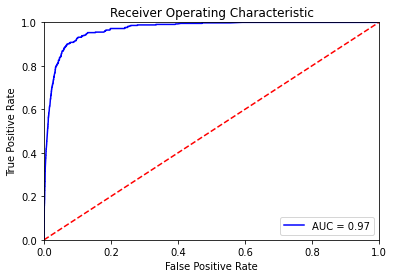
\includegraphics[width=15cm]{roc.png}
\caption{Wykres krzywej ROC. Poziomo odłożony odsetek wyników fałszywie dodatnich, pionowo odsetek wyników prawdziwie dodatnich. }
\end{figure}

\begin{figure}[H]
\centering
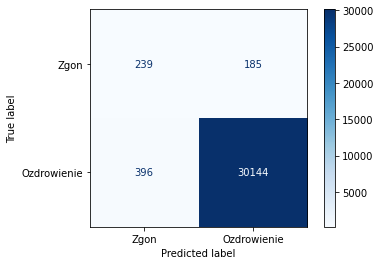
\includegraphics[width=10cm]{conf_matrix.png}
\caption{Macierz nieufności dla klas \emph{Ozdrowienie} oraz \emph{Zgon}. Poziomo odłożone wartości uzyskane przez predykcje, pionowo wartości prawdziwe. }
\end{figure}

Wysoki wynik dokładności oraz położenie krzywej ROC blisko punktu (0,1) świadczą o wysokiej jakości opracowanego modelu. Niestety, wynik F1-score oraz analiza macierzy nieufności dostarczają przeciwnych wniosków. Niższe wyniki tych miar są w pewnym stopniu spowodowane przez niezbalansowany zbiór danych. Klasa \emph{Ozdrowienie} stanowi 98,6\% wszystkich obserwacji zmiennej \emph{death\_yn} co prowadzi do niedoszacowania przez model klasy \emph{Zgon}. W celu weryfikacji tego założenia skonstruowano zbalansowany zbiór testowy i na nim przeprowadzono dodatkową predykcje. 

\begin{figure}[H]
\centering
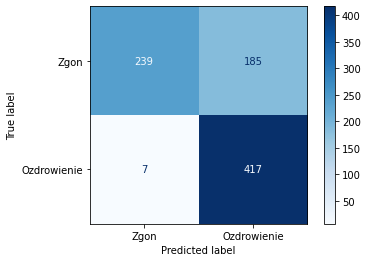
\includegraphics[width=10cm]{conf_matrix_balanced.png}
\caption{Macierz nieufności dla klas \emph{Ozdrowienie} oraz \emph{Zgon} - zbalansowany zbiór testowy.}
\end{figure}

Przy użyciu zbalansowanego zbioru testowego wartość F1-score wzrosła do 0,716. Wysoka wartość obserwacji fałszywie negatywnych świadczy o wcześniej przypuszczanym niedoszacowaniu przez model klasy \emph{Zgon}.

Kolejnym aspektem, który mógł wpłynąć na niski wynik F1-score jest niewystarczająca ilość istotnych zmiennych. Szczegółowe charakterystyki biologiczne pacjenta oraz przekrojowe zmienne środowiskowe mogą przez niewielkie odchylenia stać się kluczowe w procesie rekonwalescencji pacjentów. Przez ograniczone zasoby upublicznionych danych, a także zawężone możliwości obliczeniowe, opracowanie wysokiej klasy modelu dla wybranego problemu okazuję się zadaniem blisko nieosiągalnym.

\subsection{Interpretacja modelu}

Po skonstruowaniu optymalnego modelu uczenia maszynowego przystąpiono do etapu jego interpretacji. W tym kroku wykorzystano metodę SHAP (SHapley Additive exPlanations). W pierwszej kolejności obliczono wartość Shapleya dla wszystkich zmiennych w każdej obserwacji. 

\begin{figure}[H]
\centering
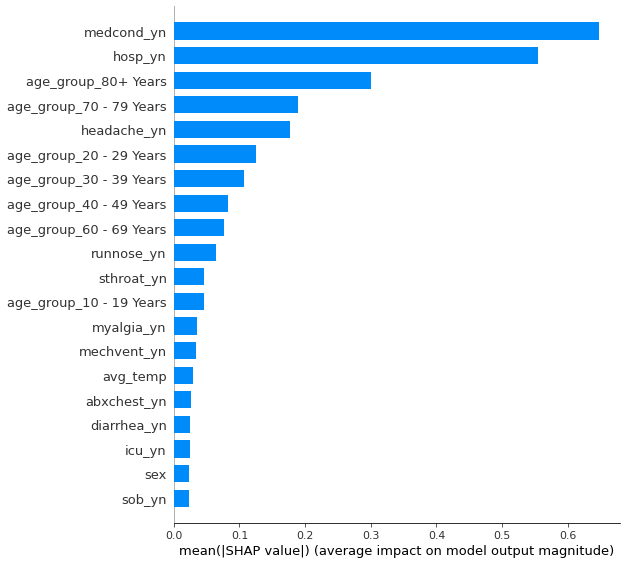
\includegraphics[width=10cm]{shap_abs.png}
\caption{Średnie z bezwzględnych wartości SHAP  - wielkości oddziaływania zmiennych na wynik modelu.}
\end{figure}

Dzięki przeprowadzonym obliczeniom wyłoniono zbiór zmiennych, które najsilniej oddziaływały na wynik modelu. Najbardziej istotną zmienną objaśniającą okazała się \emph{medcond\_yn} ze średnią bezwzględnych wartości SHAP na poziomie 0,648. Kolejną silnie wpływającą na model zmienną okazała się \emph{medcond\_yn} (średnia z bezwzględnych wartości SHAP = 0,555). Silnie oddziałującymi na wynik modelu okazały się również przedziały wiekowe, a w szczególności przedziały krańcowe. Znaczący wpływ miały również objawy występujący przy zachorowaniu przy czym najbardziej najbardziej istotną zmienną była \emph{headache\_yn} (średnia z bezwzględnych wartości SHAP = 0,176). Mniejszy wpływ miały zmienne atmosferyczne, dane demografic
zne oraz zmienne biologiczne takie jak grupa etniczna czy płeć.

\begin{figure}[H]
\centering
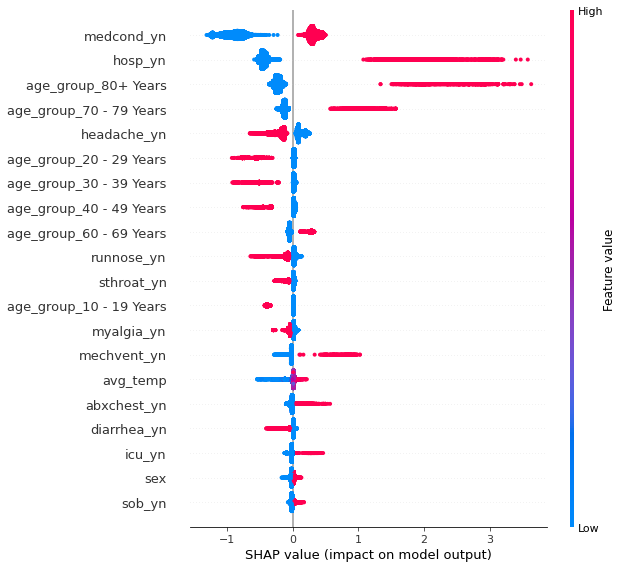
\includegraphics[width=15cm]{shap_summary.png}
\caption{Rozkłady wartości SHAP z uwzględnieniem wartości zmiennych. Kolor czerwony wskazuję na wysoką wartość zmiennej, niebieski na niską wartość zmiennej.}
\end{figure}

Kolejną zaletą wartości SHAP jest możliwość interpretacji kierunku wpływu zmiennych na wynik predykcji modelu. Z przeprowadzonych obliczeń wynika, iż zarówno zmienna \emph{medcond\_yn} jak i \emph{hosp\_yn} przy wartości 1 wpływa podwyższa prawdopodobieństwo pozytywnego wynik predykcji. Warto zauważyć, że zmienna \emph{medcond\_yn} przy wartości 0 wpływa bardzo silnie na obniżenie prawdopodobieństwa wystąpienia pozytywnej predykcji. Analiza kolejnych rozkładów zmiennych związanych z grupą wiekową wskazuję na silny wzrost prawdopodobieństwa pozytywnego wyniku predykcji przy wzroście wieku pacjenta. Rozkład wartości SHAP dla zmiennych związanych z symptomami świadczą o małym prawdopodobieństwie uzyskania pozytywnego wyniku przy występowaniu stosunkowo lekkich objawów (zmienne: \emph{headache\_yn}, \emph{runnose\_yn} oraz \emph{sthroat\_yn}. Przeciwny rezultat dają zmienne określające ciężkie symptomy tj. \emph{abxchest\_yn} oraz \emph{sob\_yn}. Rozkład wartości SHAP dla zmiennych zmiennej \emph{sex} wskazuję na przesunięcie w kierunku pozytywnego wyniku predykcji w sytuacji gdy COVID-19 został stwierdzony u mężczyzny. Niska wartość zmiennej \emph{avg\_temp} również przyczynia się do zmniejszenia prawdopodobieństwa pozytywnego wyniku predykcji. 

\subsection{Zestawienie uzyskanych wyników z wnioskami z przywołanej literatury}

Wnioski zebrane dzięki analizie zbudowanego modelu uczenia maszynowego są w wielu przypadkach zbieżne z wnioskami badań przytoczonych w rozdziale \ref{chapter:przeglad-literatury}. Najistotniejsza zmienna modelu, którą okazała się \emph{medcond\_yn}, opisująca występowanie chorób współistniejących u pacjenta, została przytoczona zarówno w badaniu \emph{Racial disparities in patients with coronavirus disease 2019 infection and gynecologic malignancy} oraz \emph{Radiographic severity index in COVID-19 pneumonia: relationship to age and sex in 783 Italian patients}. Autorzy obydwóch tych badań uwzględniają znaczący wpływ tej cechy na dalszy przebieg choroby. Kolejną zbieżną obserwacją jest znacząca dodatnia korelacja wieku pacjenta z prawdopodobieństwem zgonu pacjenta z rozpoznanym COVID-19. Wniosek ten został wyciągnięty w dwóch uprzednio wymienionych badaniach. Wysoce istotna zmienna dla modelu \emph{abxchest\_yn}, opisująca nieprawidłowości wykryte przez RTG klatki, została we wspomnianym  włoskim badaniu uznana za najważniejszą cechę rokującą dalszy przebieg choroby. Kolejnym wnioskiem z tego projektu był wpływ płci pacjenta na prawdopodobieństwo zgonu pacjenta. Wyniki tego badania oraz wnioski płynące dzięki analizie sporządzonego modelu wskazują, iż większe prawdopodobieństwo zgonu odnotowuję się dla płci męskiej. Zarówno w badaniu \emph{Effect of meteorological factors on COVID-19 cases in Bangladesh} oraz dzięki sporządzonemu modelowi uzyskano podobne wnioski na temat wpływu średniej dobowej temperatury na nasilenie wirusa SARS‑CoV‑2. Zawarte informacje w obydwóch przypadkach wskazuję na dodatnią korelacje pomiędzy tymi zmiennymi.

Niektóre wnioski badań nie uzyskały potwierdzenia w zestawieniu z wynikami uzyskanymi przez analizę sporządzonego modelu. Jednym z takich wniosków jest wpływ rasy i etniczności na przebieg choroby COVID-19 postulowany w przytoczonym badaniu wykonanym w Nowym Yorku (USA). Zmienne związane z rasą i etnicznością okazały się najmniej istotne dla wyniku predykcji opracowanego modelu. Podobnie miała się większość zmiennych atmosferycznych. W przytoczonym badaniu przeprowadzonym na terytorium Bangladeszu wnioskowano o nasileniu wirusa przy określonych warunkach pogodowych. Jednocześnie warto zauważyć, iż z analizy opracowanego modelu wynika iż jedyną zmienną, która zauważalnie wpływa na wynik modelu jest średnia dobowa temperatura. Pozostałe zmienne atmosferyczne miały niski lub pomijalny wpływ na wynik modelu.



% --- chapter ---------------------------------------------------------
\clearpage
\section{Zakończenie}


- podsumowanie pracy \\


% --- chapter -------
--------------------------------------------------
\clearpage
\section{Literatura}



% --- appendices ------------------------------------------------------
\appendix

% ---------------------------------------------------------------------
\clearpage
\section{Dodatek: Ważne rzeczy do dodania}
 



% --- bibliography ----------------------------------------------------
\clearpage
\bibliographystyle{agsm}
\bibliography{refs.bib}

% --- abstract --------------------------------------------------------
\clearpage
\addcontentsline{toc}{section}{Lista tablic}
\listoftables

% --- abstract --------------------------------------------------------
\clearpage
\addcontentsline{toc}{section}{Lista rysunków}
\listoffigures



% --- abstract --------------------------------------------------------
\clearpage
\addcontentsline{toc}{section}{Streszczenie}
\section*{Streszczenie}

Tutaj zamieszczają Państwo streszczenie pracy. Streszczenie powinno być długości około pół strony.


\end{document}

%%% Local Variables:
%%% mode: latex
%%% TeX-master: t
%%% End:
